\section{Roadmap}
\label{sec:roadmap}

\subsection{Reconciled position}
\status{INFERRED}

\pathref{README.md} marks Phase~1 (core LMS) complete and Phases~2--4 unchecked, yet discussions and feedback are already implemented -- the README has drifted (K-03). The reconciled position: the core learning lifecycle is implemented and covered by an integration test; engagement, instructor-platform and advanced-platform items remain a mix of present and absent.

\subsection{Phased plan}
\status{RECOMMENDED (not committed scope)}

\textbf{Next (hardening):} fix K-01/K-02 scoring and grade consistency, guard seed data, adopt versioned migrations, add CI gates, rotate secrets, reconcile README. \textbf{Engagement:} notifications, learning analytics, improved learner dashboard. \textbf{Instructor platform:} authoring UX, lesson management, performance analytics. \textbf{Advanced:} certificate verification, search/filtering, recommendations, password recovery, monitoring, scalable deployment. CONTRACT.md section 5.2 exclusions (payments, live classes, mobile, AI tutoring, SSO, multi-tenancy) require formal agreement before work begins.

\begin{figure}[H]
\centering
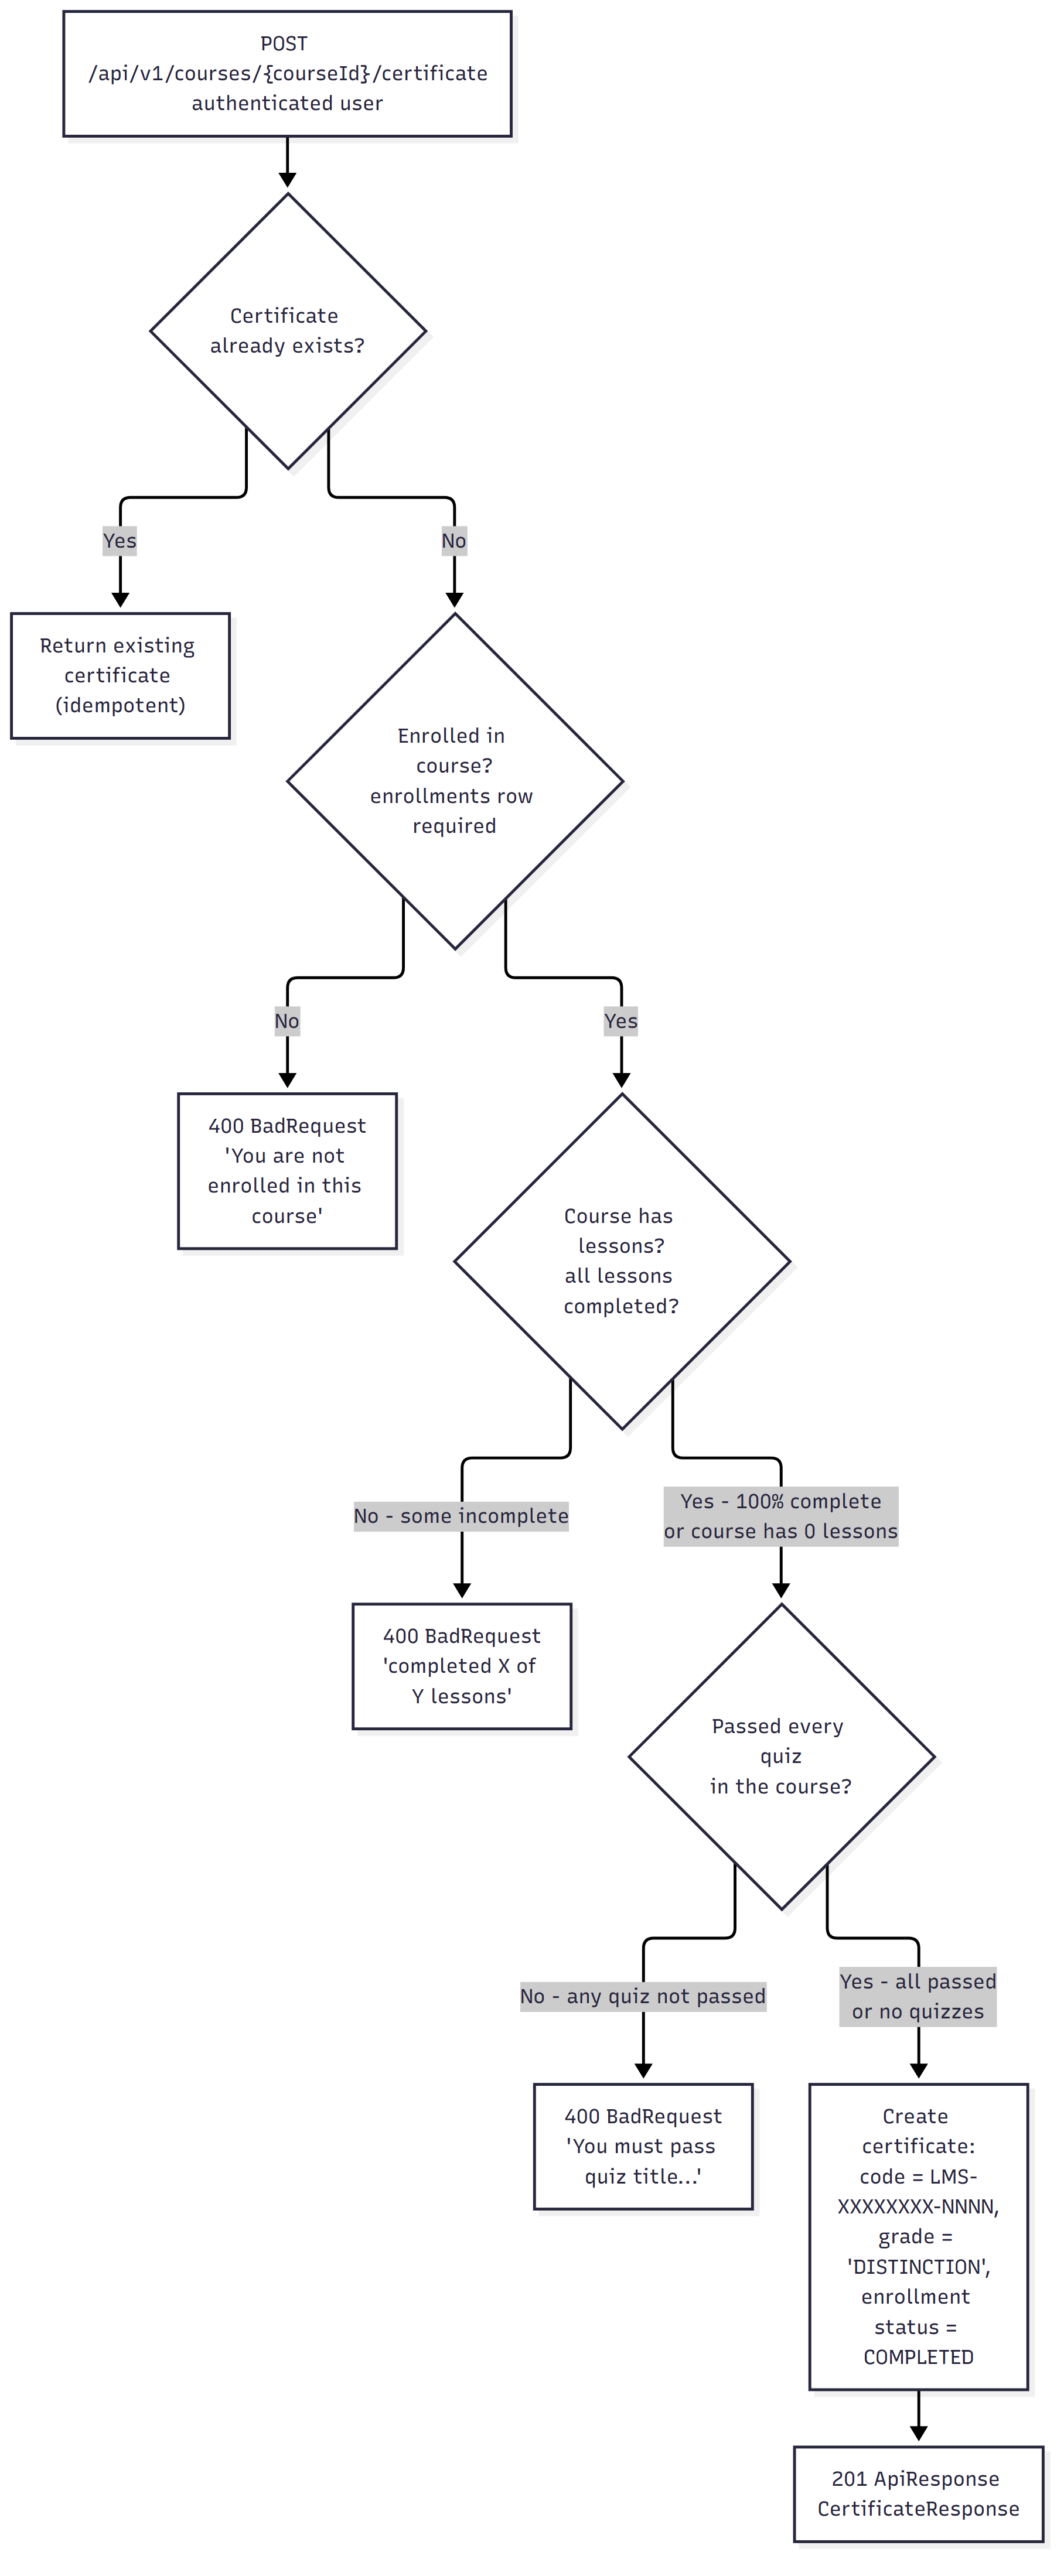
\includegraphics[width=0.9\textwidth]{diagrams/certificate-eligibility.png}
\caption{Certificate eligibility -- the gate all roadmap completion work must preserve}
\label{fig:cert-elig}
\end{figure}
